% !TeX program = xelatex
% ============================================================
% 2008 年·普通高等学校招生考试·江西卷·理科 · 简答版
% 由 tools/make_editions.py 生成（重跑会覆盖本文件）；
% 题目/解析内容在 questions.tex / answers*.tex，勿在本文件内写内容。
% ============================================================
\documentclass[zihao=-4, a4paper]{ctexart}
% ============================================================
% common/preamble.tex —— 拆分版试卷项目 · 公共导言区
% 引擎：XeLaTeX；文档类 ctexart 由各版本壳文件自行声明
% 由合并书 math-gaokao-2017-2026/preamble.tex 改造而来：
%   - 页眉左右改为可重定义宏 \gkheadL / \gkheadR（各版本壳设置）
%   - hyperref 不再写死 pdftitle（壳内 \hypersetup 覆盖）
%   - 删除书籍专用的 \chaptermark 重定义与 \gkpaper 装配宏
% ============================================================

% ---------- 数学 ----------
\usepackage{amsmath}
\usepackage{amssymb}
\usepackage{mathtools}

% ---------- 绘图 ----------
\usepackage{tikz}
\usetikzlibrary{shapes.geometric, arrows.meta, calc, patterns, angles, quotes, positioning}
\usepackage{pgfplots}
\pgfplotsset{compat=1.18}

% ---------- 版面 ----------
\usepackage{geometry}
\usepackage{needspace}
\geometry{a4paper, margin=2.2cm, headheight=15pt}
% 紧凑版式（如印刷版）可在壳文件中于 \begin{document} 前再次调用 \geometry 覆盖
\usepackage{enumitem}
\setlist{itemsep=2pt, topsep=4pt, parsep=0pt}

% 中文与行内公式混排的断行弹性：
% emergencystretch 允许段落末路不通时追加伸展量；
% 降低二元/关系符罚分，允许行内长公式在 = 、+ 等处断行（否则整段外溢）
\emergencystretch=2em
\binoppenalty=700
\relpenalty=500
\usepackage{booktabs}      % 三线表
\usepackage[most]{tcolorbox}

% ---------- 选择题选项对齐 ----------
% tasks 宏包：\begin{gkopts}(列数) \task ... \end{gkopts}
% 自动等宽分栏，选项天然对齐；列数已由内容片段按选项长度写定（4/2/1）
\usepackage{tasks}
\settasks{label={}, label-width=0pt, item-indent=1.2em,
          column-sep=1em, after-item-skip=2pt, before-skip=2pt, after-skip=4pt}
\NewTasksEnvironment[style=itemize]{gkopts}[\task](4)

% ---------- 页眉页脚 ----------
\newcommand{\gkheadL}{}   % 左页眉：卷名（壳文件 \renewcommand 设置）
\newcommand{\gkheadR}{}   % 右页眉：版本名（壳文件 \renewcommand 设置）
\usepackage{fancyhdr}
\pagestyle{fancy}
\fancyhf{}
\fancyhead[L]{\small\gkheadL}
\fancyhead[R]{\small\gkheadR}
\fancyfoot[C]{\small —— 第 \thepage\ 页 ——}
\renewcommand{\headrulewidth}{0.4pt}

% ---------- 超链接（须最后加载）----------
\usepackage{hyperref}
\hypersetup{colorlinks=true, linkcolor=blue!55!black,
            bookmarksnumbered=true, unicode=true}

% ============================================================
% common/macros.tex —— 自定义命令与环境（题号、解析头、提示框等）
% 与合并书 math-gaokao-2017-2026/preamble.tex 的自定义段保持一致，
% 保证内容片段（questions.tex / answers.tex）在两个项目间可互换。
% ============================================================

% ---------- 试卷标识（壳文件 \renewcommand 设置，用于 label 命名空间）----------
\newcommand{\gkpaperid}{none}

% ---------- 题号 ----------
% 试题部分的题号：加粗编号 + 自动 \label{q:<卷id>:<题号>}
\newcommand{\gkti}[1]{\par\medskip\noindent
  \textbf{#1．}\phantomsection\label{q:\gkpaperid:#1}\ignorespaces}
% 多卷/分部重启题号时，#1 是唯一内部顺序号（交叉引用身份），#2 才是原卷显示题号。
\newcommand{\gktiwithlabel}[2]{\par\medskip\noindent
  \textbf{#2．}\phantomsection\label{q:\gkpaperid:#1}\ignorespaces}

% 解析部分的题头：小标题 + 回链到试题页
% （仅在题目与解析同文档的版本中回链有效；试题版不含解析头，无悬空引用）
\newcommand{\gksolhead}[2]{%
  \Needspace{3\baselineskip}\subsubsection*{第 #1 题\if\relax\detokenize{#2}\relax\else（#2）\fi}%
  \phantomsection\label{s:\gkpaperid:#1}%
  {\small\color{gray}（题目见第~\pageref{q:\gkpaperid:#1}~页）}\par\nopagebreak}
% 与 \gktiwithlabel 成对：显示原题号，但回链仍用唯一内部顺序号。
\newcommand{\gksolheadwithlabel}[3]{%
  \Needspace{3\baselineskip}\subsubsection*{第 #2 题\if\relax\detokenize{#3}\relax\else（#3）\fi}%
  \phantomsection\label{s:\gkpaperid:#1}%
  {\small\color{gray}（题目见第~\pageref{q:\gkpaperid:#1}~页）}\par\nopagebreak}

% ---------- 填空题空位 ----------
\newcommand{\gkblank}{\underline{\hspace{2.2em}}}

% ---------- 提示框 ----------
% 卷种提示 / 解析归属声明（醒目，浅黄）
\newtcolorbox{gknotice}{colback=yellow!8, colframe=orange!60!black,
  boxrule=0.5pt, arc=1.5pt, left=6pt, right=6pt, top=4pt, bottom=4pt,
  before skip=8pt, after skip=8pt}

% 方法提示 / 注（浅蓝，用于解析后的点评与题量说明）
\newtcolorbox{gktip}{colback=blue!4, colframe=blue!35!black,
  boxrule=0.4pt, arc=1.5pt, left=6pt, right=6pt, top=4pt, bottom=4pt,
  before skip=6pt, after skip=6pt, fontupper=\small}

% ---------- 答案行 ----------
% 解析中独立成段的"答案：X"用带底色的行呈现
\newcommand{\gkanswer}[1]{\par\smallskip\noindent
  \tcbox[width=\linewidth, tcbox width=auto limited,
         colback=green!6, colframe=green!35!black, boxrule=0.4pt,
         arc=1.5pt, left=4pt, right=4pt, top=2pt, bottom=2pt,
         nobeforeafter]{\textbf{#1}}\par\smallskip}

% ---------- 结构标题 ----------
% 结构标题后通常紧跟一个带 0.5\textheight 起始预留的解析题块；0.4 只够放标题，
% 会把下一题整体推到下一页，留下孤立的「二、填空题」等页尾标题。
\newcommand{\gkpart}[1]{\Needspace{0.6\textheight}\subsection*{#1}\nopagebreak}     % 标题 + 首题
% （一）必考题 / 解析小问标题：块式加粗段，可自动换行（\paragraph 的 run-in 版式会溢出）
\newcommand{\gksubpart}[1]{\Needspace{6\baselineskip}\par\medskip\noindent\textbf{#1}\par\nopagebreak\smallskip}

% 罗马数字Ⅰ-Ⅻ（U+2160）与圈号①②③（U+2460）划入 CJK 字符类，
% 用中文字体渲染——西文字体 Latin Modern 缺这些字形，否则整段静默丢字
\xeCJKDeclareCharClass{CJK}{"2160 -> "217F, "2460 -> "24FF}

% ============================================================
% common/questions_env.tex —— 题目 / 解析的语义包装环境
%
% questions.tex 中每道题包在 \begin{question}...\end{question} 里，
% answers.tex 中每题解析包在 \begin{answer}...\end{answer} 里；
% 题头排版仍由内容行中的 \gkti / \gksolhead 完成（见 macros.tex）。
%
% 环境本身不产生任何盒子或垂直间距（只引入一个 TeX 分组），
% 排版结果与不包裹时逐点一致。它的价值在于：
%   1. 给每道题一个机器可数的结构边界（校验脚本数环境数 = 题量）；
%   2. 为将来的条件编译留钩子——某版本可重定义环境实现按题取舍。
% ============================================================

% 环境不把整题装盒：题目与解析仍可自然跨页，但开始题块前必须为题面、
% 图形/表格或解析首段留出足够空间。仅保留 2 个 baseline 会让题干、
% 选项和图形在页边界处被拆开，形成不可打印的孤立内容；题目保留
% 0.15\textheight，在避免短题制造大段空白与避免题块拆分之间取平衡。
% 解析题块保留 0.5\textheight，以容纳“题面 + 图形/选项 + 首段解析”；
% 结构标题仍用更大的保留量；末页自然收尾由视觉复审判定。
\newenvironment{question}{\Needspace{0.15\textheight}}{}
\newenvironment{answer}{\Needspace{0.5\textheight}}{}

\renewcommand{\gkpaperid}{gk-2008-jiangxi-science}
\renewcommand{\gkheadL}{2008 年·普通高等学校招生考试·江西卷·理科 · 数学}
\renewcommand{\gkheadR}{简答版}
\hypersetup{pdftitle={2008 年·普通高等学校招生考试·江西卷·理科 数学 · 简答版}}
\begin{document}
\begin{center}
  {\Large\bfseries 2008 年·普通高等学校招生考试·江西卷·理科}\\[4pt]
  {\large 数学 · 简答版}
\end{center}
\medskip
\pdfbookmark[1]{试题}{sec:q}
% questions.tex —— 2008 年·普通高等学校招生考试·江西卷·理科 · 题目内容片段（无答案）
% 由 tools/generate_projects.py 依来源总账自 2008/2008_数学真题_江西理_试题.md 生成，勿手改（改源 MD 后重跑）


\gkpart{一、选择题}

\begin{question}
\gkti{1}在复平面内，复数 $z=\sin2+\mathrm i\cos2$ 对应的点位于（　）

（A）第一象限

（B）第二象限

（C）第三象限

（D）第四象限

\end{question}
\begin{question}
\gkti{2}定义集合运算：$A*B=\{z\mid z=xy,\ x\in A,\ y\in B\}$。设 $A=\{1,2\}$，$B=\{0,2\}$，则集合 $A*B$ 的所有元素之和为（　）

（A）$0$

（B）$2$

（C）$3$

（D）$6$

\end{question}
\begin{question}
\gkti{3}若函数 $y=f(x)$ 的值域是 $\left[\dfrac12,3\right]$，则函数 $F(x)=f(x)+\dfrac1{f(x)}$ 的值域是（　）

（A）$\left[\dfrac12,3\right]$

（B）$\left[2,\dfrac{10}3\right]$

（C）$\left[\dfrac52,\dfrac{10}3\right]$

（D）$\left[3,\dfrac{10}3\right]$

\end{question}
\begin{question}
\gkti{4}$\lim\limits_{x\to1}\dfrac{\sqrt{x+3}-2}{\sqrt x-1}=$（　）

（A）$\dfrac12$

（B）$0$

（C）$-\dfrac12$

（D）不存在

\end{question}
\begin{question}
\gkti{5}在数列 $\{a_n\}$ 中，$a_1=2$，$a_{n+1}=a_n+\ln\left(1+\dfrac1n\right)$，则 $a_n=$（　）

（A）$2+\ln n$

（B）$2+(n-1)\ln n$

（C）$2+n\ln n$

（D）$1+n+\ln n$

\Needspace{0.4\textheight}
\end{question}
\begin{question}
\gkti{6}函数 $y=\tan x+\sin x-|\tan x-\sin x|$ 在区间 $\left(\dfrac{\pi}2,\dfrac{3\pi}2\right)$ 内的图象大致是（　）

（四个选项为下列四个图象，依次对应 (A)、(B)、(C)、(D)。）
\nopagebreak[4]
\begin{center}% 2008 年江西卷理科第 6 题：y=tan x+sin x-|tan x-sin x| 在 (π/2,3π/2) 内的四个候选图象。
% 来源 PDF：gaokaomath-src/普通高考/2008/2008江西文.pdf
% SHA-256：8d079d71fadf20911ed2fd71acfe9562b94eb962cfe5228fe7a376f3b599b239
% 原页：2008江西理.pdf 第 1 页（A3 三栏）第 1 栏，书页码 459。
% 绘制依据：由 |tan x - sin x| 分段，x∈(π/2,π) 时 y=2tan x（负值升到 0），
%   x∈(π,3π/2) 时 y=2sin x（由 0 降到 -2）。四个候选按原页 2×2 排布，
%   坐标刻度取 π/2→1、π→2、3π/2→3（单位长度相同），π/2 与 3π/2 的标号用白底压住虚线。
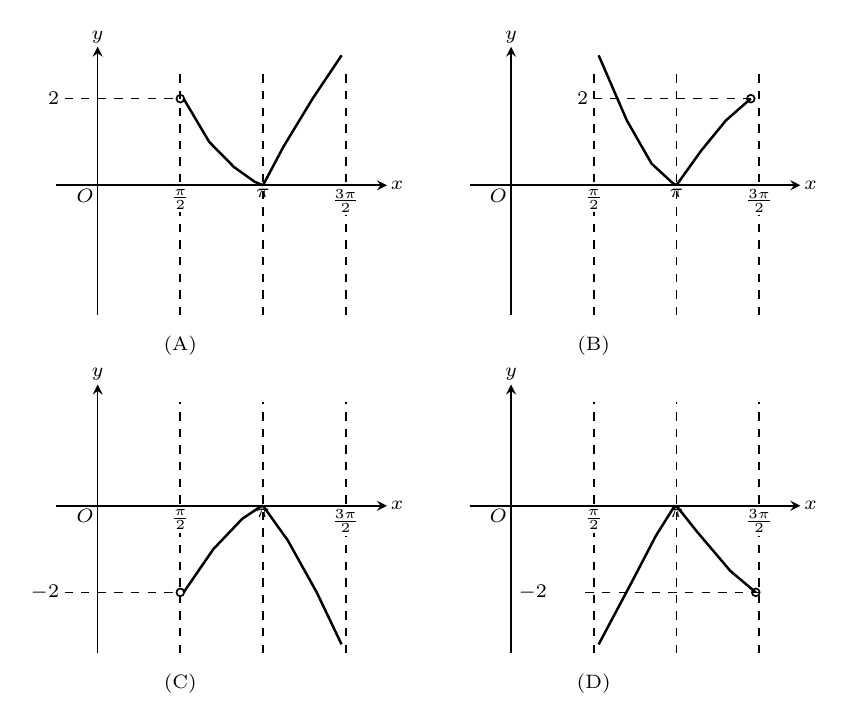
\begin{tikzpicture}[x=1.05cm, y=0.55cm, semithick, font=\scriptsize,
  every node/.style={inner sep=1.1pt}]

  % ---------- (A) ----------
  \begin{scope}[shift={(0,0)}]
    \draw[->,>=stealth] (-0.5,0) -- (3.5,0) node[right] {$x$};
    \draw[->,>=stealth] (0,-3.0) -- (0,3.2) node[above] {$y$};
    \node[below left] at (0,0) {$O$};
    \draw[dashed] (1.0,-3.0) -- (1.0,2.6);
    \draw[dashed] (2.0,-3.0) -- (2.0,2.6);
    \draw[dashed] (3.0,-3.0) -- (3.0,2.6);
    \node[below, fill=white] at (1.0,0) {$\frac{\pi}{2}$};
    \node[below] at (2.0,0) {$\pi$};
    \node[below, fill=white] at (3.0,0) {$\frac{3\pi}{2}$};
    \draw[dashed] (-0.4,2.0) -- (1.0,2.0);
    \node[left] at (-0.42,2.0) {$2$};
    \draw (1.0,2.0) circle (1.4pt);
    \draw[line width=0.9pt] plot coordinates {(1.04,2.0) (1.35,1.0) (1.65,0.42) (1.9,0.08) (2.0,0.0)};
    \draw[line width=0.9pt] plot coordinates {(2.0,0.0) (2.25,0.9) (2.6,2.0) (2.95,3.0)};
    \node at (1.0,-3.7) {(A)};
  \end{scope}

  % ---------- (B) ----------
  \begin{scope}[shift={(5.0,0)}]
    \draw[->,>=stealth] (-0.5,0) -- (3.5,0) node[right] {$x$};
    \draw[->,>=stealth] (0,-3.0) -- (0,3.2) node[above] {$y$};
    \node[below left] at (0,0) {$O$};
    \draw[dashed] (1.0,-3.0) -- (1.0,2.6);
    \draw[dashed] (2.0,-3.0) -- (2.0,2.6);
    \draw[dashed] (3.0,-3.0) -- (3.0,2.6);
    \node[below, fill=white] at (1.0,0) {$\frac{\pi}{2}$};
    \node[below] at (2.0,0) {$\pi$};
    \node[below, fill=white] at (3.0,0) {$\frac{3\pi}{2}$};
    \draw[dashed] (1.0,2.0) -- (2.9,2.0);
    \node[left] at (0.98,2.0) {$2$};
    \draw[line width=0.9pt] plot coordinates {(1.06,3.0) (1.4,1.5) (1.7,0.5) (1.95,0.06) (2.0,0.0)};
    \draw[line width=0.9pt] plot coordinates {(2.0,0.0) (2.3,0.8) (2.6,1.5) (2.9,2.0)};
    \draw (2.9,2.0) circle (1.4pt);
    \node at (1.0,-3.7) {(B)};
  \end{scope}

  % ---------- (C) ----------
  \begin{scope}[shift={(0,-7.4)}]
    \draw[->,>=stealth] (-0.5,0) -- (3.5,0) node[right] {$x$};
    \draw[->,>=stealth] (0,-3.4) -- (0,2.8) node[above] {$y$};
    \node[below left] at (0,0) {$O$};
    \draw[dashed] (1.0,-3.4) -- (1.0,2.4);
    \draw[dashed] (2.0,-3.4) -- (2.0,2.4);
    \draw[dashed] (3.0,-3.4) -- (3.0,2.4);
    \node[below, fill=white] at (1.0,0) {$\frac{\pi}{2}$};
    \node[below] at (2.0,0) {$\pi$};
    \node[below, fill=white] at (3.0,0) {$\frac{3\pi}{2}$};
    \draw[dashed] (-0.4,-2.0) -- (1.0,-2.0);
    \node[left] at (-0.42,-2.0) {$-2$};
    \draw (1.0,-2.0) circle (1.4pt);
    \draw[line width=0.9pt] plot coordinates {(1.04,-2.0) (1.4,-1.0) (1.75,-0.3) (1.97,-0.02) (2.0,0.0)};
    \draw[line width=0.9pt] plot coordinates {(2.0,0.0) (2.3,-0.8) (2.65,-2.0) (2.95,-3.2)};
    \node at (1.0,-4.1) {(C)};
  \end{scope}

  % ---------- (D) ----------
  \begin{scope}[shift={(5.0,-7.4)}]
    \draw[->,>=stealth] (-0.5,0) -- (3.5,0) node[right] {$x$};
    \draw[->,>=stealth] (0,-3.4) -- (0,2.8) node[above] {$y$};
    \node[below left] at (0,0) {$O$};
    \draw[dashed] (1.0,-3.4) -- (1.0,2.4);
    \draw[dashed] (2.0,-3.4) -- (2.0,2.4);
    \draw[dashed] (3.0,-3.4) -- (3.0,2.4);
    \node[below, fill=white] at (1.0,0) {$\frac{\pi}{2}$};
    \node[below] at (2.0,0) {$\pi$};
    \node[below, fill=white] at (3.0,0) {$\frac{3\pi}{2}$};
    \draw[dashed] (0.9,-2.0) -- (3.1,-2.0);
    \node[left] at (0.48,-2.0) {$-2$};
    \draw[line width=0.9pt] plot coordinates {(1.06,-3.2) (1.45,-1.8) (1.75,-0.7) (1.96,-0.06) (2.0,0.0)};
    \draw[line width=0.9pt] plot coordinates {(2.0,0.0) (2.25,-0.6) (2.65,-1.5) (2.96,-2.0)};
    \draw (2.96,-2.0) circle (1.4pt);
    \node at (1.0,-4.1) {(D)};
  \end{scope}
\end{tikzpicture}
\end{center}
\nopagebreak[4]
\end{question}
\begin{question}
\gkti{7}已知 $F_1$、$F_2$ 是椭圆的两个焦点，满足 $\overrightarrow{MF_1}\cdot\overrightarrow{MF_2}=0$ 的点 $M$ 总在椭圆内部，则椭圆离心率的取值范围是（　）

（A）$(0,1)$

（B）$\left(0,\dfrac12\right]$

（C）$\left(0,\dfrac{\sqrt2}2\right)$

（D）$\left[\dfrac{\sqrt2}2,1\right)$

\end{question}
\begin{question}
\gkti{8}$(1+\sqrt[3]x)^6\left(1+\dfrac1{\sqrt[4]x}\right)^{10}$ 展开式中的常数项为（　）

（A）$1$

（B）$46$

（C）$4245$

（D）$4246$

\end{question}
\begin{question}
\gkti{9}若 $0<a_1<a_2$，$0<b_1<b_2$，且 $a_1+a_2=b_1+b_2=1$，则下列代数式中值最大的是（　）

（A）$a_1b_1+a_2b_2$

（B）$a_1a_2+b_1b_2$

（C）$a_1b_2+a_2b_1$

（D）$\dfrac12$

\end{question}
\begin{question}
\gkti{10}连结球面上两点的线段称为球的弦。半径为 $4$ 的球的两条弦 $AB$、$CD$ 的长度分别等于 $2\sqrt7$、$4\sqrt3$，$M$、$N$ 分别为 $AB$、$CD$ 的中点，每条弦的两端都在球面上运动，有下列四个命题：

① 弦 $AB$、$CD$ 可能相交于点 $M$；

② 弦 $AB$、$CD$ 可能相交于点 $N$；

③ $MN$ 的最大值为 $5$；

④ $MN$ 的最小值为 $1$。

其中真命题的个数为（　）

（A）$1$ 个

（B）$2$ 个

（C）$3$ 个

（D）$4$ 个

\end{question}
\begin{question}
\gkti{11}电子钟一天显示的时间是从 $00\!:\!00$ 到 $23\!:\!59$，每一时刻都由四个数字组成，则一天中任一时刻显示的四个数字之和为 $23$ 的概率为（　）

（A）$\dfrac1{180}$

（B）$\dfrac1{288}$

（C）$\dfrac1{360}$

（D）$\dfrac1{480}$

\end{question}
\begin{question}
\gkti{12}已知函数 $f(x)=2mx^2-2(4-m)x+1$，$g(x)=mx$，若对于任一实数 $x$，$f(x)$ 与 $g(x)$ 的值至少有一个为正数，则实数 $m$ 的取值范围是（　）

（A）$(0,2)$

（B）$(0,8)$

（C）$(2,8)$

（D）$(-\infty,0)$

\end{question}
\gkpart{二、填空题}

\begin{question}
\gkti{13}直角坐标平面内三点 $A(1,2)$，$B(3,-2)$，$C(9,7)$，若 $E$、$F$ 为线段 $BC$ 的三等分点，则 $\overrightarrow{AE}\cdot\overrightarrow{AF}=$\gkblank{}。

\end{question}
\begin{question}
\gkti{14}不等式 $2^{x^2-3x+1}\leqslant\dfrac12$ 的解集为\gkblank{}。

\end{question}
\begin{question}
\gkti{15}过抛物线 $x^2=2py$（$p>0$）的焦点 $F$ 作倾斜角为 $30^\circ$ 的直线，与抛物线分别交于 $A$、$B$ 两点（点 $A$ 在 $y$ 轴左侧），则 $\dfrac{|AF|}{|FB|}=$\gkblank{}。

\Needspace{0.4\textheight}
\end{question}
\begin{question}
\gkti{16}如图 1，一个正四棱柱形的密闭容器水平放置，其底部镶嵌了同底的正四棱锥形实心装饰块，容器内盛有 $a$ 升水时，水面恰好经过正四棱锥的顶点 $P$。如果将容器倒置，水面也恰好过点 $P$（图 2）。有下列四个命题：

\begin{gkopts}(1)
\task A．正四棱锥的高等于正四棱柱高的一半；
\task B．将容器侧面水平放置时，水面也恰好过点 $P$；
\task C．任意摆放该容器，当水面静止时，水面都恰好经过点 $P$；
\task D．若往容器内再注入 $a$ 升水，则容器恰好能装满。
\end{gkopts}

其中真命题的代号是\gkblank{}。（写出所有真命题的代号）
\nopagebreak[4]
\begin{center}% 2008 年江西卷理科第 16 题：正四棱柱容器内底部镶嵌同底的正四棱锥（顶点 P），水面恰好过 P；
%   图 1 为水平放置，图 2 为倒置后水面同样过 P。
% 来源 PDF：gaokaomath-src/普通高考/2008/2008江西理.pdf
% SHA-256：8d079d71fadf20911ed2fd71acfe9562b94eb962cfe5228fe7a376f3b599b239
% 原页：2008江西理.pdf 第 1 页（A3 三栏）第 3 栏，书页码 459。
% 绘制依据：棱柱高取 5、棱锥高取 3（正好一半略多，仅作示意）。斜投影下底面为 A(0,0)、B(3,0)、
%   C(4.2,0.9)、D(1.2,0.9)。图 1：棱锥底面贴底、顶点 P 在底面中心上方高 3 处，水面过 P；
%   图 2：容器倒置，棱锥顶点朝下，水面同样过 P。水用浅灰填充。
\begin{tikzpicture}[scale=0.52, semithick, every node/.style={inner sep=1.2pt, font=\small}]

  % ---------- 图 1：正放 ----------
  \begin{scope}[shift={(0,0)}]
    \coordinate (A)  at (0,0);
    \coordinate (B)  at (3,0);
    \coordinate (C)  at (4.2,0.9);
    \coordinate (D)  at (1.2,0.9);
    \coordinate (A1) at (0,5);
    \coordinate (B1) at (3,5);
    \coordinate (C1) at (4.2,5.9);
    \coordinate (D1) at (1.2,5.9);
    \coordinate (P)  at (2.1,3.45);

    % 水（低于水面的部分）
    \fill[gray!22] (0,0) -- (3,0) -- (4.2,0.9) -- (1.2,0.9) -- cycle;
    \fill[gray!22] (0,3) -- (3,3) -- (4.2,3.9) -- (1.2,3.9) -- cycle;

    % 棱柱
    \draw (A) -- (B) -- (C) -- (C1) -- (B1) -- (A1) -- cycle;
    \draw (B) -- (B1);
    \draw (C) -- (C1);
    \draw[dashed] (A1) -- (D1) -- (C1);
    \draw[dashed] (A) -- (D) -- (C);
    \draw[dashed] (D) -- (D1);

    % 内嵌正四棱锥（底面为 ABCD，顶点 P 在上）
    \draw[dashed] (A) -- (P);
    \draw[dashed] (B) -- (P);
    \draw[dashed] (C) -- (P);
    \draw[dashed] (D) -- (P);

    % 水面
    \draw[line width=0.8pt] (0,3) -- (3,3) -- (4.2,3.9) -- (1.2,3.9) -- cycle;

    \fill (P) circle (2pt);
    \node[right=1pt] at (P) {$P$};
    \node[below] at (2.1,-0.8) {图 1};
  \end{scope}

  % ---------- 图 2：倒置 ----------
  \begin{scope}[shift={(7.6,0)}]
    \coordinate (A2)  at (0,0);
    \coordinate (B2)  at (3,0);
    \coordinate (C2)  at (4.2,0.9);
    \coordinate (D2)  at (1.2,0.9);
    \coordinate (A3) at (0,5);
    \coordinate (B3) at (3,5);
    \coordinate (C3) at (4.2,5.9);
    \coordinate (D3) at (1.2,5.9);
    \coordinate (P2) at (2.1,1.55);

    % 水（低于水面的部分；倒置后棱锥顶点朝下）
    \fill[gray!22] (0,0) -- (3,0) -- (4.2,0.9) -- (1.2,0.9) -- cycle;
    \fill[gray!22] (0,1.1) -- (3,1.1) -- (4.2,2.0) -- (1.2,2.0) -- cycle;

    % 棱柱
    \draw (A2) -- (B2) -- (C2) -- (C3) -- (B3) -- (A3) -- cycle;
    \draw (B2) -- (B3);
    \draw (C2) -- (C3);
    \draw[dashed] (A3) -- (D3) -- (C3);
    \draw[dashed] (A2) -- (D2) -- (C2);
    \draw[dashed] (D2) -- (D3);

    % 内嵌正四棱锥（倒置后顶点 P2 朝下）
    \draw[dashed] (A3) -- (P2);
    \draw[dashed] (B3) -- (P2);
    \draw[dashed] (C3) -- (P2);
    \draw[dashed] (D3) -- (P2);

    % 水面
    \draw[line width=0.8pt] (0,1.1) -- (3,1.1) -- (4.2,2.0) -- (1.2,2.0) -- cycle;

    \fill (P2) circle (2pt);
    \node[right=1pt] at (P2) {$P$};
    \node[below] at (2.1,-0.8) {图 2};
  \end{scope}
\end{tikzpicture}
\end{center}
\nopagebreak[4]
\end{question}
\gkpart{三、解答题}

\begin{question}
\gkti{17}在 $\triangle ABC$ 中，$a$、$b$、$c$ 分别为角 $A$、$B$、$C$ 所对的边长，$a=2\sqrt3$，$\tan\dfrac{A+B}2+\tan\dfrac C2=4$，$\sin B\sin C=\cos^2\dfrac A2$。求 $A$、$B$ 及 $b$、$c$。

\end{question}
\begin{question}
\gkti{18}因冰雪灾害，某柑桔基地果林严重受损，为此有关专家提出两种拯救果树的方案，每种方案都需分两年实施。若实施方案一，预计第一年可以使柑桔产量恢复到灾前的 $1.0$ 倍、$0.9$ 倍、$0.8$ 倍的概率分别是 $0.3$、$0.3$、$0.4$；第二年可以使柑桔产量为第一年产量的 $1.25$ 倍、$1.0$ 倍的概率分别是 $0.5$、$0.5$。若实施方案二，预计第一年可以使柑桔产量达到灾前的 $1.2$ 倍、$1.0$ 倍、$0.88$ 倍的概率分别是 $0.2$、$0.3$、$0.5$；第二年可以使柑桔产量为第一年产量的 $1.2$ 倍、$1.0$ 倍的概率分别是 $0.4$、$0.6$。实施每种方案第一年与第二年相互独立，令 $\xi_i$（$i=1,2$）表示方案 $i$ 实施两年后柑桔产量达到灾前产量的倍数。

（1）写出 $\xi_1$、$\xi_2$ 的分布列；

（2）实施哪种方案，两年后柑桔产量超过灾前产量的概率更大？

（3）不管哪种方案，如果实施两年后柑桔产量达不到、恰好达到、超过灾前产量，预计利润分别为 $10$ 万元、$15$ 万元、$20$ 万元。问实施哪种方案的平均利润更大？

\end{question}
\begin{question}
\gkti{19}等差数列 $\{a_n\}$ 各项均为正整数，$a_1=3$，前 $n$ 项和为 $S_n$，等比数列 $\{b_n\}$ 中，$b_1=1$，且 $b_2S_2=64$，$\{b_n\}$ 是公比为 $64$ 的等比数列。

（1）求 $a_n$ 与 $b_n$；

（2）证明：$\dfrac1{S_1}+\dfrac1{S_2}+\cdots+\dfrac1{S_n}<\dfrac34$。

\Needspace{0.4\textheight}
\end{question}
\begin{question}
\gkti{20}如图，正三棱锥 $O-ABC$ 的三条侧棱 $OA$、$OB$、$OC$ 两两垂直，且长度均为 $2$。$E$、$F$ 分别是 $AB$、$AC$ 的中点，$H$ 是 $EF$ 的中点，过 $EF$ 的一个平面与侧棱 $OA$、$OB$、$OC$ 或其延长线分别相交于 $A_1$、$B_1$、$C_1$，已知 $OA_1=\dfrac32$。

（1）证明：$B_1C_1\perp$ 平面 $OAH$；

（2）求二面角 $O-A_1B_1-C_1$ 的大小。
\nopagebreak[4]
\begin{center}% 2008 年江西卷理科第 20 题：正三棱锥 O-ABC，OA、OB、OC 两两垂直且长为 2；
%   E、F 为 AB、AC 中点，H 为 EF 中点；过 EF 的平面与 OA、OB、OC 的延长线交于 A1、B1、C1。
% 来源 PDF：gaokaomath-src/普通高考/2008/2008江西文.pdf
% SHA-256：8d079d71fadf20911ed2fd71acfe9562b94eb962cfe5228fe7a376f3b599b239
% 原页：2008江西理.pdf 第 2 页（A3 三栏）第 1 栏，书页码 460。
% 绘制依据：按原页斜投影：O 在上，A 在左、B 在下、C 在右；A1 在 OA 延长线上、C1 在 OC 延长线上、
%   B1 在 OB 延长线上；截面三角形 A1B1C1 为实线，EF 与 H 在内部（虚线）。
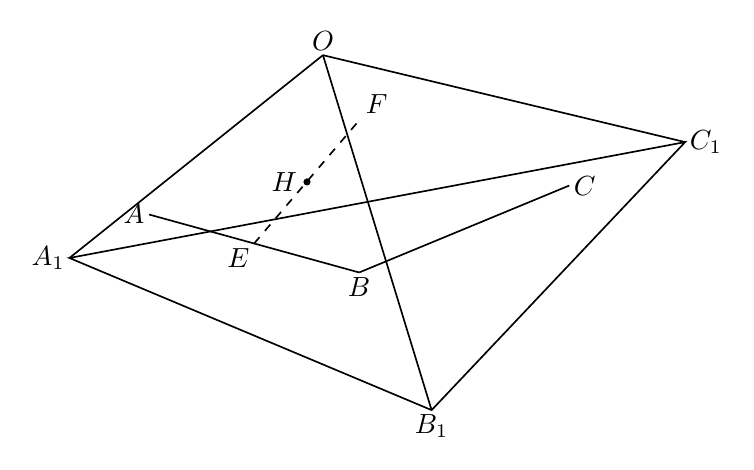
\begin{tikzpicture}[scale=0.92, semithick, every node/.style={inner sep=1.4pt}]
  \coordinate (O) at (2.60,4.30);
  \coordinate (A) at (0.20,2.10);
  \coordinate (B) at (3.10,1.30);
  \coordinate (C) at (6.00,2.50);
  \coordinate (A1) at (-0.90,1.50);
  \coordinate (B1) at (4.10,-0.60);
  \coordinate (C1) at (7.60,3.10);
  \coordinate (E) at (1.65,1.70);
  \coordinate (F) at (3.10,3.40);
  \coordinate (H) at (2.38,2.55);

  % 侧棱（延长后到 A1、B1、C1）
  \draw (O) -- (A1);
  \draw (O) -- (C1);
  \draw (O) -- (B1);

  % 截面三角形
  \draw (A1) -- (B1) -- (C1) -- cycle;

  % 底边
  \draw (A) -- (B);
  \draw (B) -- (C);

  % EF 与 H
  \draw[dashed] (E) -- (F);
  \fill (H) circle (1.4pt);

  \node[above] at (O) {$O$};
  \node[left] at (A) {$A$};
  \node[below] at (B) {$B$};
  \node[right] at (C) {$C$};
  \node[left] at (A1) {$A_1$};
  \node[below] at (B1) {$B_1$};
  \node[right] at (C1) {$C_1$};
  \node[below left] at (E) {$E$};
  \node[above right=1pt] at (F) {$F$};
  \node[left=2pt] at (H) {$H$};
\end{tikzpicture}
\end{center}
\nopagebreak[4]
\Needspace{0.4\textheight}
\end{question}
\begin{question}
\gkti{21}设点 $P(x_0,y_0)$ 在直线 $x=m$（$y\neq\pm m$，$0<m<1$）上，过点 $P$ 作双曲线 $x^2-y^2=1$ 的两条切线 $PA$、$PB$，切点为 $A$、$B$，定点 $M\left(\dfrac1m,0\right)$。

（1）过点 $A$ 作直线 $x-y=0$ 的垂线，垂足为 $N$，试求 $\triangle AMN$ 的重心 $G$ 所在的曲线方程；

（2）求证：$A$、$M$、$B$ 三点共线。
\nopagebreak[4]
\begin{center}% 2008 年江西卷理科第 21 题：双曲线 x^2-y^2=1，点 P 在直线 x=m（0<m<1）上，过 P 的两条切线与双曲线
%   相切于 A、B，定点 M(1/m,0)；过 A 作直线 x-y=0 的垂线，垂足为 N。
% 来源 PDF：gaokaomath-src/普通高考/2008/2008江西理.pdf
% SHA-256：8d079d71fadf20911ed2fd71acfe9562b94eb962cfe5228fe7a376f3b599b239
% 原页：2008江西理.pdf 第 2 页（A3 三栏）第 2 栏，书页码 460。
% 绘制依据：取 m=1/2，P(1/2,-2)。切点弦为 mx-y0y=1，即 x/2+2y=1，与 x^2-y^2=1 交于
%   A(1.029,0.243)（右支上侧）与 B(-1.296,0.824)（左支上侧）；M(2,0)；
%   N 为 A 到直线 y=x 的垂足，N=((x_A+y_A)/2,(x_A+y_A)/2)=(0.636,0.636)。
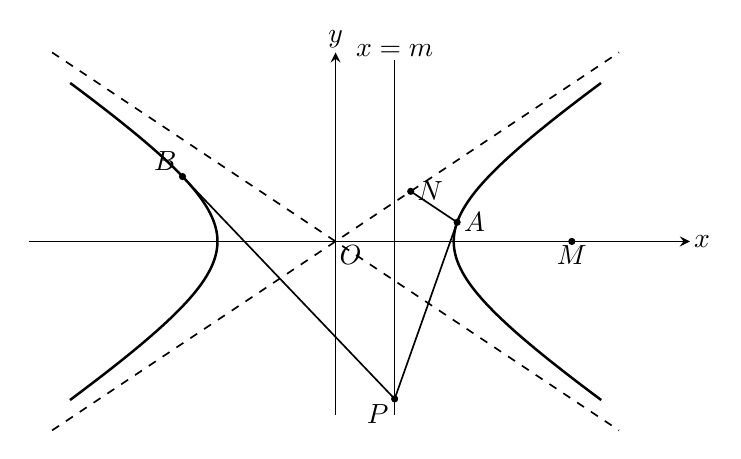
\begin{tikzpicture}[x=1.5cm, y=1.0cm, semithick, every node/.style={inner sep=1.2pt}]
  \draw[->,>=stealth] (-2.6,0) -- (3.0,0) node[right] {$x$};
  \draw[->,>=stealth] (0,-2.2) -- (0,2.4) node[above] {$y$};
  \node[below right] at (0,0) {$O$};

  % 渐近线
  \draw[dashed] (-2.4,-2.4) -- (2.4,2.4);
  \draw[dashed] (-2.4,2.4) -- (2.4,-2.4);

  % 双曲线两支
  \draw[line width=0.9pt, domain=-1.45:1.45, samples=80] plot ({cosh(\x)},{sinh(\x)});
  \draw[line width=0.9pt, domain=-1.45:1.45, samples=80] plot ({-cosh(\x)},{sinh(\x)});

  \coordinate (A) at (1.029,0.243);
  \coordinate (B) at (-1.296,0.824);
  \coordinate (P) at (0.5,-2);
  \coordinate (M) at (2,0);
  \coordinate (N) at (0.636,0.636);

  % 直线 x=m
  \draw (0.5,-2.2) -- (0.5,2.3);
  \node[above] at (0.5,2.3) {$x=m$};

  % 两条切线
  \draw (P) -- (A);
  \draw (P) -- (B);

  % A 到 y=x 的垂线，垂足 N
  \draw (A) -- (N);

  \fill (P) circle (1.3pt); \node[below left=1pt] at (P) {$P$};
  \fill (A) circle (1.3pt); \node[right=1pt] at (A) {$A$};
  \fill (B) circle (1.3pt); \node[above left=1pt] at (B) {$B$};
  \fill (M) circle (1.3pt); \node[below] at (M) {$M$};
  \fill (N) circle (1.3pt); \node[right=1pt] at (N) {$N$};
\end{tikzpicture}
\end{center}
\nopagebreak[4]
\end{question}
\begin{question}
\gkti{22}已知函数 $f(x)=\dfrac1{\sqrt{1+x}}+\dfrac1{\sqrt{1+a}}+\sqrt{\dfrac{ax}{ax+8}}$，$x\in(0,+\infty)$。

（1）当 $a=8$ 时，求 $f(x)$ 的单调区间；

（2）对任意正数 $a$，证明：$1<f(x)<2$。

\end{question}
\clearpage
\pdfbookmark[1]{答案速查}{sec:a}
\Needspace{8\baselineskip}
\begin{center}{\Large\bfseries 答案速查}\end{center}
\medskip
% answers_short.tex —— 2008 年·普通高等学校招生考试·江西卷·理科 · 简短答案速查
% 由 tools/make_short_answers.py 自 answers.tex 的 \gksolhead/\gkanswer 提取，
% 并与 2008/2008_数学真题_江西理_答案要点.md 逐题比对后生成，勿手改（改源 MD 后重跑）。

\begin{gknotice}
\textbf{使用说明}：本节只给最终答案便于快速核对，完整推导见解析版。答案为编写者独立推导，\textbf{非官方标准答案}。
\end{gknotice}

\gkpart{选择题}
\begin{center}\begin{tabular}{ccccccccccccc}
\toprule
题号 & 1 & 2 & 3 & 4 & 5 & 6 & 7 & 8 & 9 & 10 & 11 & 12 \\
\midrule
答案 & B & D & B & A & A & D & C & C & A & C & C & B \\
\bottomrule
\end{tabular}\end{center}

\gkpart{填空题}
\begin{itemize}[leftmargin=2.6em]
  \item[\textbf{13.}] $22$。
  \item[\textbf{14.}] $[1,2]$。
  \item[\textbf{15.}] $\dfrac13$。
  \item[\textbf{16.}] D。
\end{itemize}

\gkpart{解答题}
\begin{itemize}[leftmargin=2.6em]
  \item[\textbf{17.}] $A=120^\circ$，$B=C=30^\circ$，$b=c=2$。
  \item[\textbf{18.}] （1）分布列如下；（2）方案二；（3）方案二。
  \item[\textbf{19.}] 【源疑点】按题面条件无解。
  \item[\textbf{20.}] （1）证明见解析；（2）$\arccos\dfrac{\sqrt6}6$。
  \item[\textbf{21.}] （1）$\left(x-\dfrac1{3m}\right)^2-y^2=\dfrac29$；（2）证明见解析。
  \item[\textbf{22.}] （1）增区间 $(0,1)$，减区间 $(1,+\infty)$；（2）证明见解析。
\end{itemize}

\end{document}
